\documentclass[11pt]{article}
\usepackage{geometry,marginnote} % Pour passer au format A4
\geometry{hmargin=1cm, vmargin=1.5cm} % 

% Page et encodage
\usepackage[T1]{fontenc} % Use 8-bit encoding that has 256 glyphs
\usepackage[english,french]{babel} % Français et anglais
\usepackage[utf8]{inputenc} 

\usepackage{lmodern}
\usepackage[np]{numprint}
\setlength\parindent{0pt}

% Graphiques
\usepackage{graphicx,float,grffile}
\usepackage{tikz,pst-eucl,pst-plot,pstricks,pst-node,pstricks-add,pst-fun,pgfplots} 

% Maths et divers
\usepackage{amsmath,amsfonts,amssymb,amsthm,verbatim,scratch3}
\usepackage{multicol,enumitem,url,eurosym,gensymb,tabularx}

\DeclareUnicodeCharacter{20AC}{\euro}



% Sections
\usepackage{sectsty} % Allows customizing section commands
\allsectionsfont{\centering \normalfont\scshape}

% Tête et pied de page
\usepackage{fancyhdr} \pagestyle{fancy} \fancyhead{} \fancyfoot{}

%\fancyfoot[L]{Collège Faubert}
%\fancyfoot[C]{\thepage / 6}
%\fancyfoot[R]{Série Générale}

\renewcommand{\headrulewidth}{0pt} % Remove header underlines
%\renewcommand{\footrulewidth}{0pt} % Remove footer underlines

\newcommand{\horrule}[1]{\rule{\linewidth}{#1}} % Create horizontal rule command with 1 argument of height

\newcommand{\Pointilles}[1][3]{%
  \multido{}{#1}{\makebox[\linewidth]{\dotfill}\\[\parskip]
}}

\newtheorem{Definition}{Définition}

\usepackage{siunitx}
\sisetup{
    detect-all,
    output-decimal-marker={,},
    group-minimum-digits = 3,
    group-separator={~},
    number-unit-separator={~},
    inter-unit-product={~}
}

\setlength{\columnseprule}{1pt}


\begin{document}

\textbf{Nom, Prénom :} \hspace{8cm} \textbf{Classe :} \hspace{3cm} \textbf{Date :}\\

\begin{center}
  \textit{Les propositions mathématiques sont reçues comme vraies parce que personne n’a intérêt qu’elles soient fausses.} - \textbf{Montesquieu}
\end{center}

\subsection*{Définitions}

\textbf{Périmètre : } \dotfill \\ \Pointilles[1] 

\textbf{Aire : } \dotfill \\ \Pointilles[1] 

\subsection*{ex1 - Aire}

\begin{figure}[H]
  \centering
  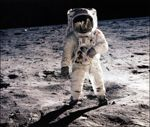
\includegraphics[width=0.8\linewidth]{6x7-aires-perimetres/ex1.pdf}
\end{figure}

\begin{enumerate}
  \item[1.] \textbf{Aire figure 1 :} \dotfill
  \item[2.] \textbf{Aire figure 2 : } \dotfill
  \item[3.] \textbf{Aire figure 3 : } \dotfill
  \item[4.] \textbf{Aire figure 4 : } \dotfill
  \item[5.] \textbf{Aire figure 5 : } \dotfill
\end{enumerate}

\subsection*{ex2 - Périmètre}

\begin{multicols}{2} 
\begin{enumerate}
  \item[1.] Mesurer à la règle le périmètre de la figure ci-contre. \\
  Écrire la longueurs de chaque côté.
\end{enumerate}

\textbf{Périmètre : } \dotfill \columnbreak

  \begin{figure}[H]
    \centering
    
\includegraphics[width=0.7\linewidth]{6x7-aires-perimetres/ex2.pdf}
  \end{figure}
\end{multicols}


\begin{multicols}{2} 
  \begin{enumerate}
  \item[2.] Mesurer au compas et à la règle le périmètre de la figure.\\
  Laisser les traces de construction du compas. 
\end{enumerate}

\textbf{Périmètre : } \dotfill  \columnbreak

  \begin{figure}[H]
    \centering
    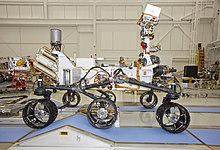
\includegraphics[width=0.7\linewidth]{6x7-aires-perimetres/ex3.pdf}
  \end{figure}
\end{multicols}

\horrule{2px} \newpage

\subsection*{ex3 - Tracer}

\begin{enumerate}
  \item[1.] Tracer à la règle et au compas le triangle de côté : AB = 8cm, AC = 5cm et BC = 4,2cm. Laisser les traces de construction.
  \item[2.] Tracer à la règle et au compas le triangle de côté : MN = 6,1cm, NP = 7.4cm et MP = 8,8cm. Laisser les traces de construction.
\end{enumerate}

\thispagestyle{empty}
\pgfplotsset{minor grid style = {dashed}}
\pgfplotsset{major grid style = {solid}}
    \begin{figure}\centering
        \begin{tikzpicture}
        \begin{axis}[grid = both,
                     ticks = none,
                     minor tick num = 1,
                     xmin = 0,
                     ymin = 0,
                     xmax = 20,
                     ymax = 16,
                     width = 20cm,
                     height = 16cm,
                     scale only axis]
        \end{axis}
        \end{tikzpicture}
    \end{figure}

\subsection*{ex4 - Convertir}

\begin{multicols}{2} 

\begin{itemize}[label={$\bullet$}]
  \item $12 \,km = \dotfill m$
  \item $9 \,m = \dotfill cm$
  \item $134 \,m = \dotfill mm$
  \item $1\, 200 \,m = \dotfill km$
  \item $245\, 000 \,mm = \dotfill m$
  \item $5\, 700 \,cm = \dotfill m$
\end{itemize} 

\begin{itemize}[label={$\bullet$}]
  \item $24 \,km^2 = \dotfill m^2$
  \item $17 \,m^2 = \dotfill cm^2$
  \item $128 \,m^2 = \dotfill mm^2$
  \item $8\, 900 \, 000 \,m^2 = \dotfill km^2$
  \item $140\, 000 \,cm^2 = \dotfill m^2$
  \item $3\, 200 \,mm^2 = \dotfill cm^2$
\end{itemize} 

\end{multicols}

\end{document}